\cleardoublepage
\counterwithout{figure}{section}
\counterwithout{table}{section} 
\counterwithout{equation}{section}
\counterwithin{figure}{chapter}
\counterwithin{table}{chapter} 
\counterwithin{equation}{chapter}


\chapter{Assignment}
\label{sec:aufgabenstellung}
 In frame of this thesis a process is to be developed for generation of the dental color shades using an inkjet printer.  The mechanic aspects of responsible for the movement are not included to the project. A stepper motor driven system responsible for the coordinated movement of the axes controlled by a SmoothieBoard v2-mini is provided by the project partner Bredent GmbH. The specifications of the printing system, like a single drop volume or the max printing distance and angle are to be determined. Afterwards an adequate droplet generator is to be selected. The diameter of the nozzle is as important as the driver technology generating the droplets, which has a direct effect on the optical resolution of the printed pattern. With piezoelectric droplet generators, smaller and faster drops are possible but electromagnetic ones are cheaper. The quantitative coloring behavior depending on the absorption characteristics of the dental ceramic is an unknown to the state of the research and the technology. The shades of the dental colors are to be brought about using the main colors with the highest saturation level and and a brightener, which is a water based diluter with  an identical composition to the inks, except lacking the metal-ionic coloring agent. The proportions of the ink and the diluter is not the only parameter affecting the shade of the generated color, but also the application sequence can have a significant effect on the optical perception. Since the translucency of the dental zirconia effects the level of color reflection, the depth of the colored section can have an undeniable effect on the natural look of the dental crown. At last the generated shades are to be verified with the existing color standards. The receipt for each single shade generation has to be prepared. The deployed droplets are not fly and settle on the contact point drying on the surface, but are expected to be absorbed and spread inside the porous material. This nature of the interaction between the ink in its fluid form and porous zirconia makes the definition of the system a nonlinear three dimensional fluid dynamics problem. A model is to be generated taking the every compensational aspect of the nonlinear ink behavior, in order to achieve a point accurate color acquisition.
 
 

\chapter{Expected Advantages and Functions of the Solution}
One of the most important advantages is quantification of the coloring process followed by the printing process. Until this day the crown coloring process is made by dental technologists all around the world. In other words all of the dental replacements are partially handcrafted. In the market hand crafted is another word for made by a craftsman, specifically for the unique owner of the product. Just as any other product on the market, the word handcrafted has a prominent effect on the price tag of the item. The word handcrafted also means the product has some tiny error, a nuance special for each unique sample. If the object of interest is a decor for the home of the consumer, it is one of the most welcome properties, but if the object of interest is an implant, which is to be carried all the time on the comsumer's body as a part of the it, the property everyone is looking for is perfection. A perfect shape, color, consistency and harmony is a standard to evaluate the quality of the work done by the dentist and of course involving the dental technologist. The quantification of the coloring process is the most important advantage of the solution, when it is considered looking from this aspect.Thus, the error can be terminated and the quality deviation can be limited to an acceptable variance. 

Another aspect to consider is the ink costs. Each of the ink bottles are labeled with the same price tag by the manufacturer. However not all of the ink bottles contain a material worth the same value actually. The shades of the colors ranging from 1 to 3.5 are only diluted versions of the bottle with the shade 4.0. Buying the most concentrated tone and diluting it is here an economical solution, as it is in every other section of the industry. Also, the whole spectrum of shades can be obtained with only 4 ink bottles and a brightener by halftone printing. The required purchase variety, transportation costs, and the space requirement are all reduced with the usage of only the most saturated shades.

\chapter{Solution Structure}
The structural concept is utilization of a 5-axis printing system. 4 base colors with the highest saturation (A,B,C and D4) are to be used with the brightener instead of 16 predefined shades. The amount of the brightener defines the shade of the color. A 3-axis table and the 2-axis nozzle holder are responsible for the coordination during the printing process.
\newline
\begin{figure}[h]
	\centering
	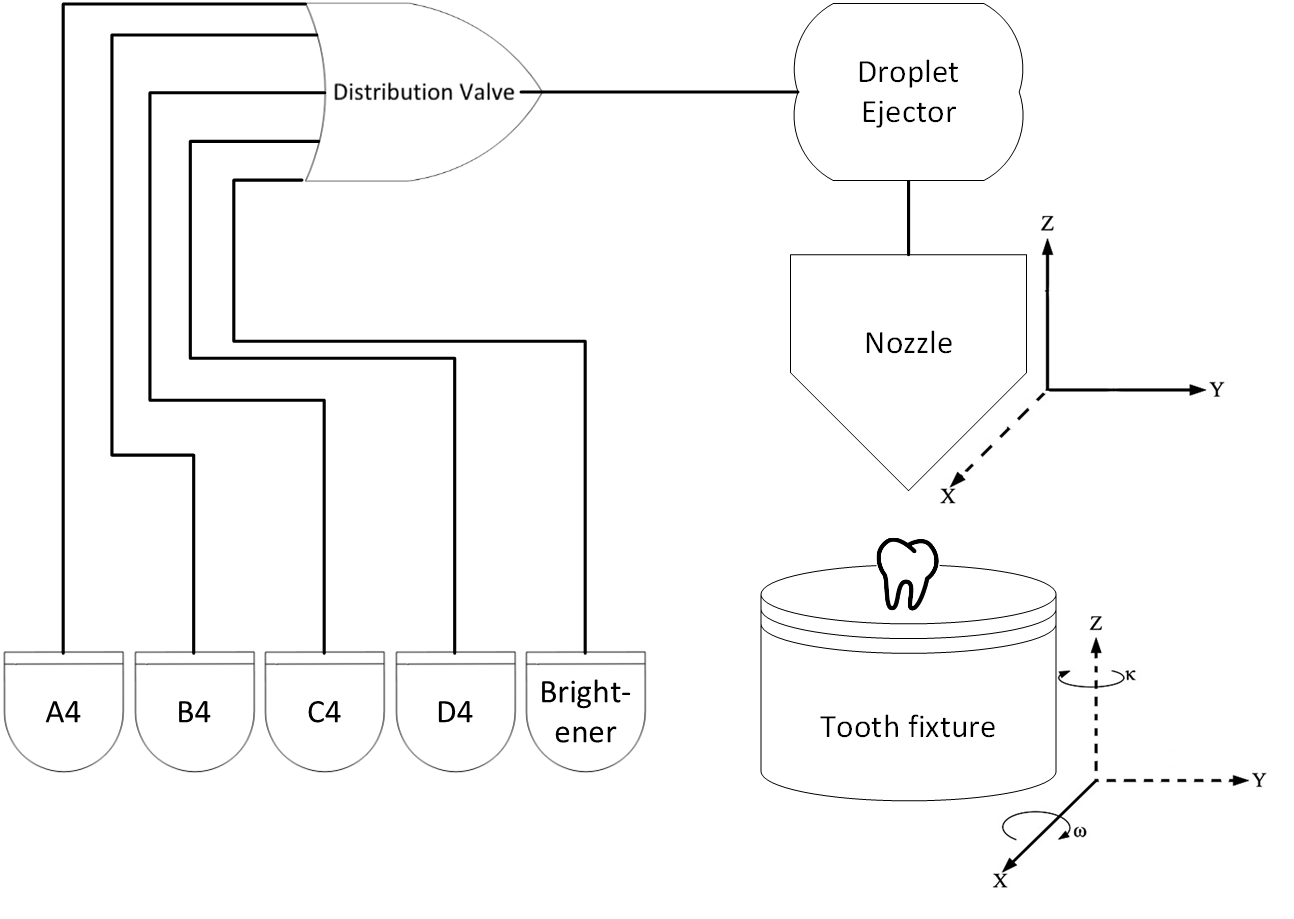
\includegraphics[width=0.9\textwidth]{grafiken/SolutionStructure.jpg}
	\caption{Solution Structure}
	\label{fig:SolutionStructure}
\end{figure} 

\chapter{Solution Processes}
\label{sec:Lösungsprozesse}
The process concept is realized in three stages. Each stage depends on the previous one and That’s the progress so far. First stage is finding the ink and ceramic properties, such as ink viscosity and surface tension, ceramic void fraction and ink absorption time. Second stage is determination of drop properties and deployment metrics, which consist of drop volume, nozzle escape velocity of the drops, the optimal distance between the nozzle and zirconia surface and the angle between the drop projectile and the surface. The aspects to be considered under the third stage color and shade acquisition are trace distance (the distance between two sequential lines on the printed surface), proximity effect, which refers to how the proximity of two colored areas affect the shade of the uncolored area in between and finally the dependency of the shade on the brightener ratio.
\newline
\begin{figure}[h]
	\centering
	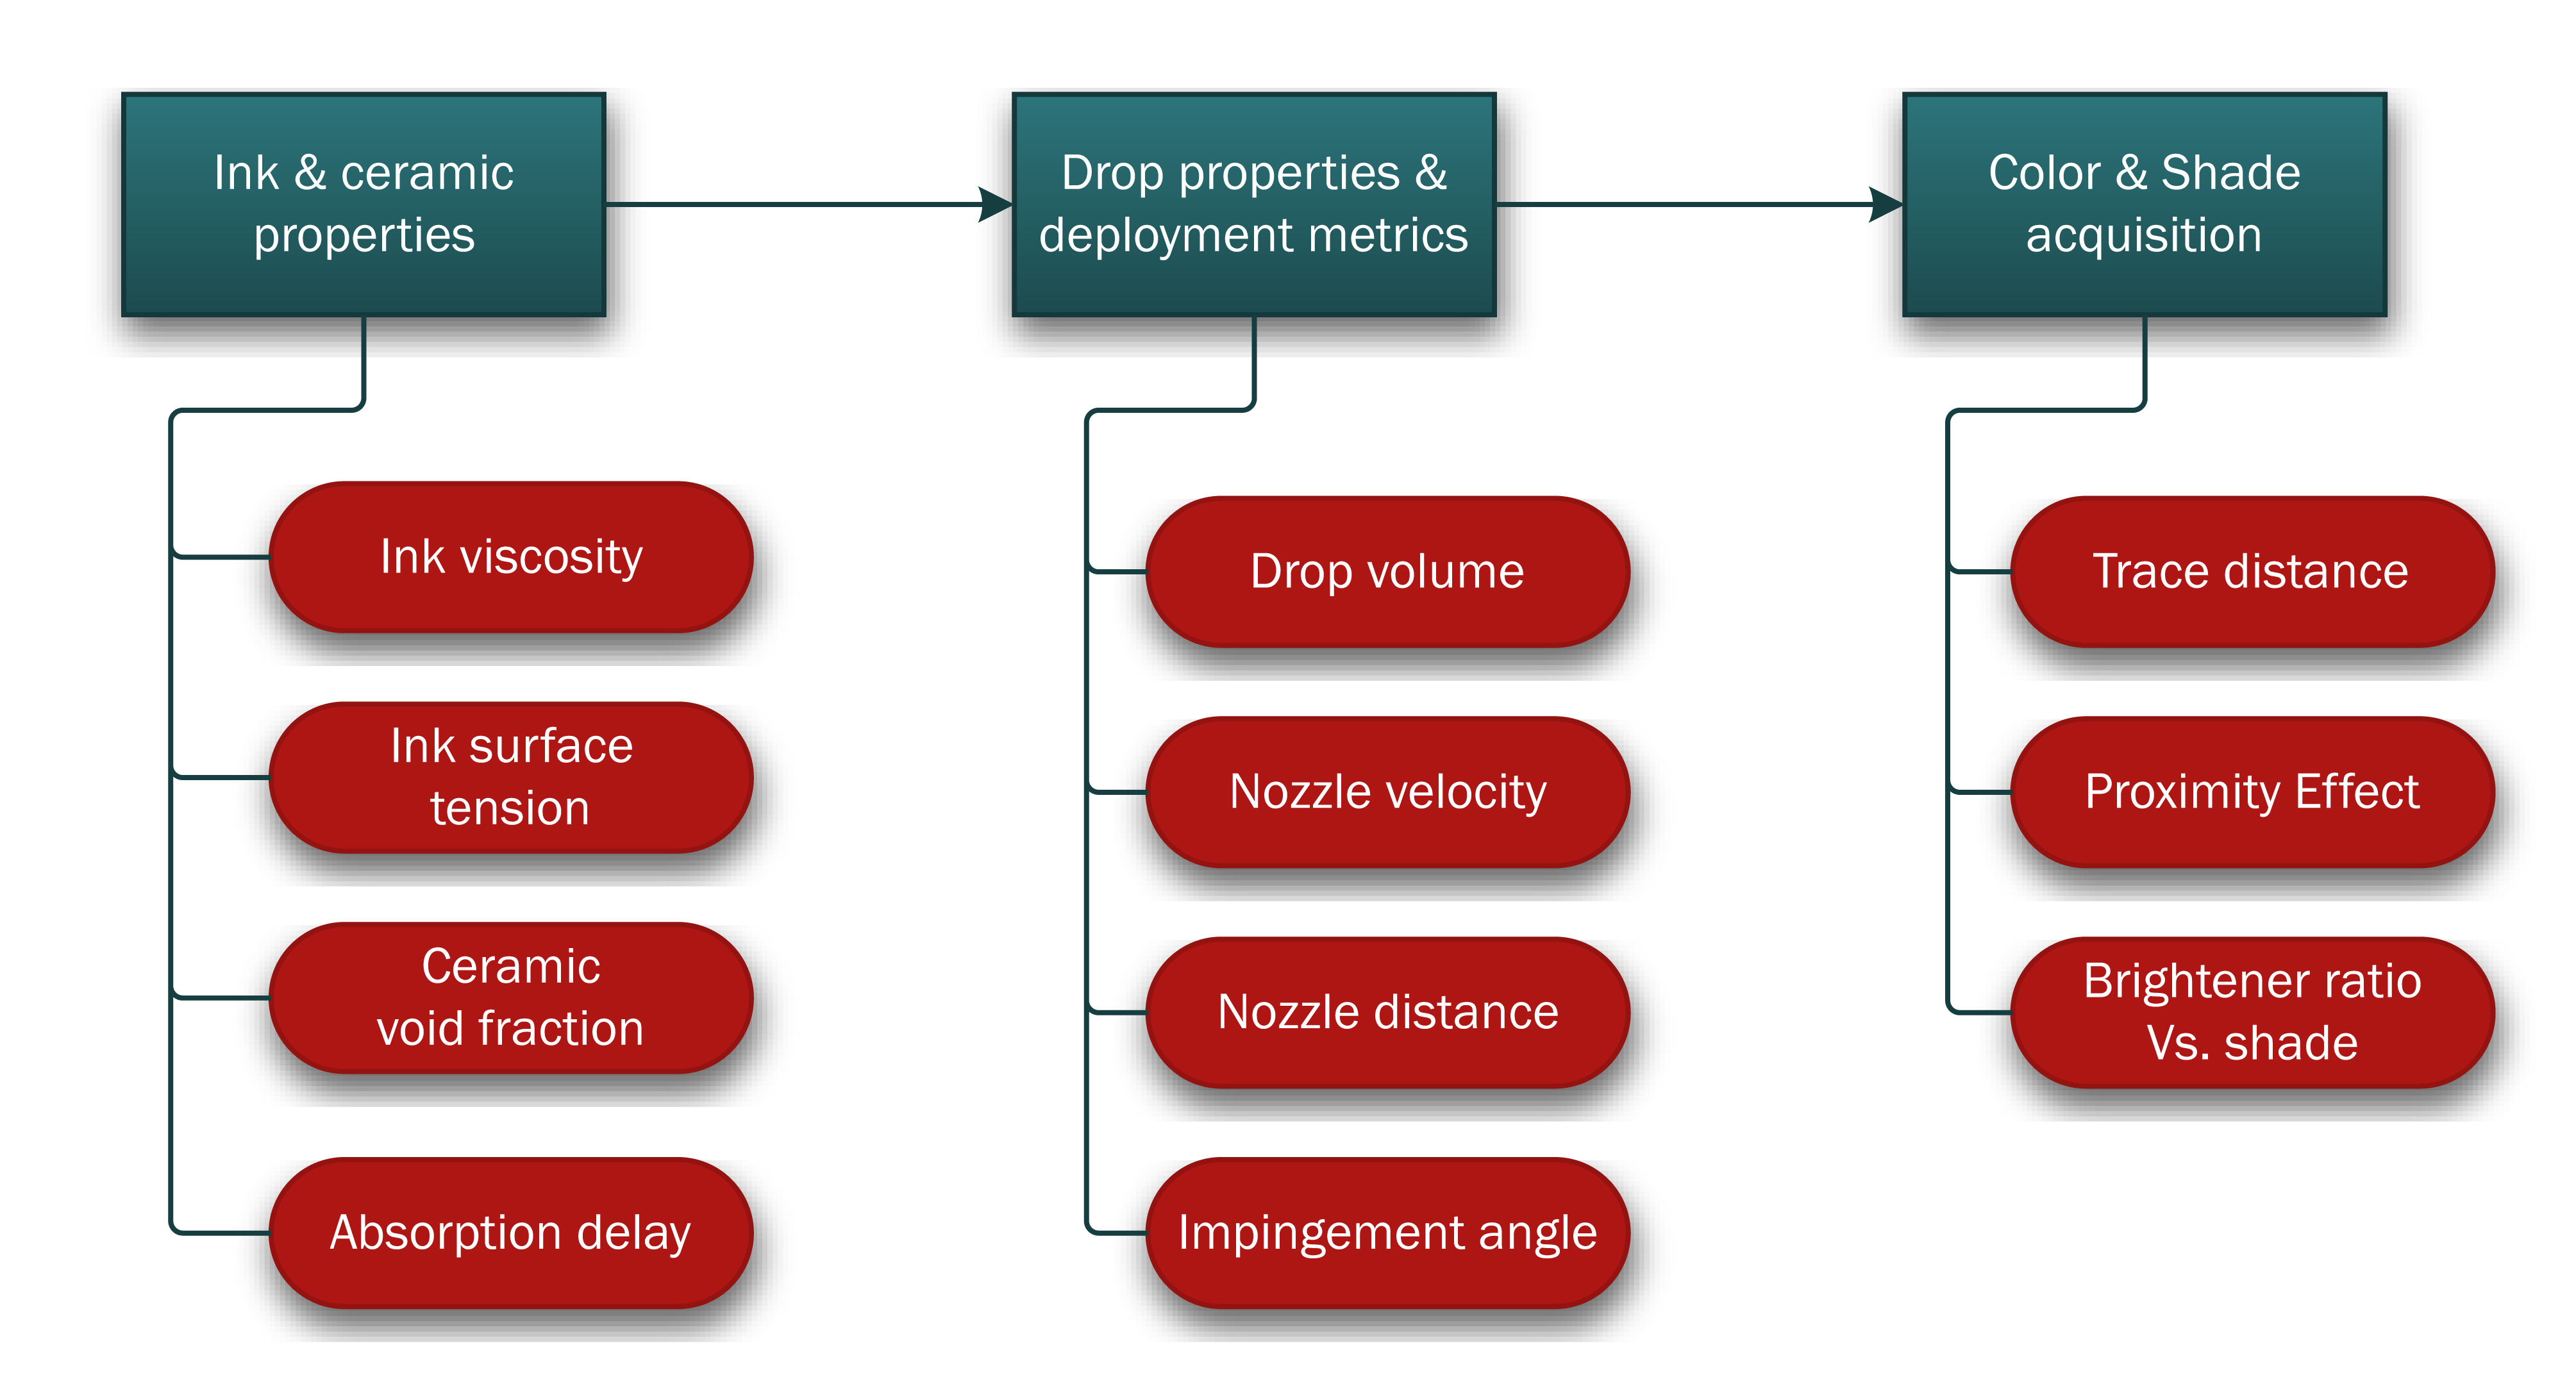
\includegraphics[width=0.9\textwidth]{grafiken/SolutionProcesses.jpg}
	\caption{Solution Processes}
	\label{fig:SolutionProcesses}
\end{figure} 


\chapter{Distinctive Features of the Solution}
\label{sec:Unterscheidungsmerkmale}
The project is the first automated printing approach in dental coloring and also the first time the shades are generated using the darkest base colors and a brightener.

\chapter{Experiments}

Before moving on to the experiments I want to show you the 5 axis printing system prototype provided by Bredent for conduction of the experiments. 
It utilizes a single nozzle printhead  with a piezoelectric valve to generate the droplets. Ink selection, positioning and drop generation commands are given with a G-Code.
\begin{figure}[h]
	\centering
	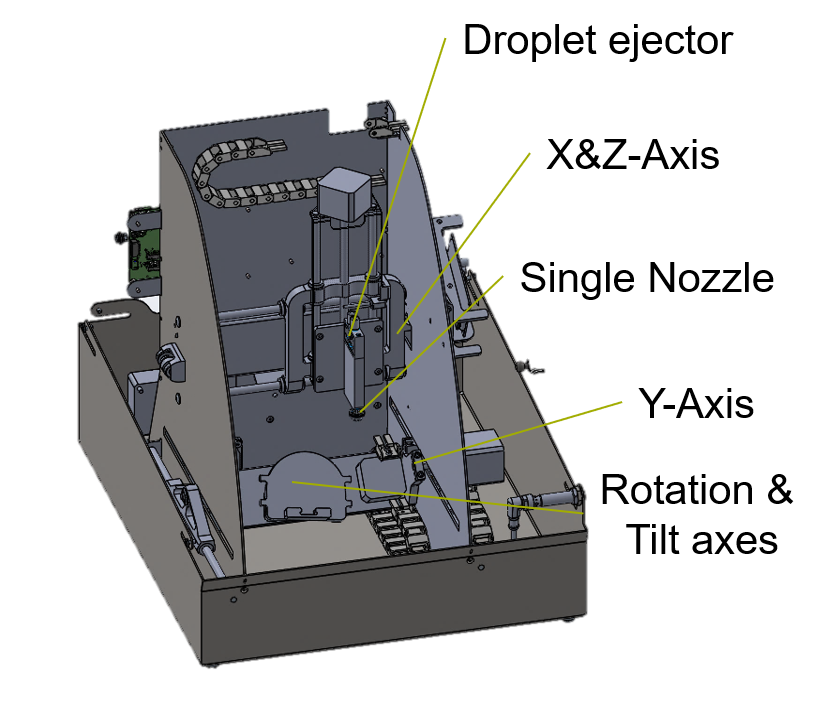
\includegraphics[width=0.7\textwidth]{grafiken/PrototypeText.png}
	\caption{5 axis printer design for dental ink (Matthias Leininger, Bredent GmbH)}
	\label{fig:Prototype}
\end{figure} 

\section{Material Properties}
For a dental technician it is totally trivial how viscous the ink is but for an automated printing  process the quantization of the properties is highly important. In the first experiment, the properties of the coloring agents A1, A2 and A3.5 are determined and compared to those of water. The inks have a similar density to water, but with increasing coloring agent the surface tension gets lower and the viscosity gets 3 times higher when compared to water.Also, a porosity measurement for the zirconia is conducted, which revealed a 43 percent void fraction.
\begin{figure}[h]
	\centering
	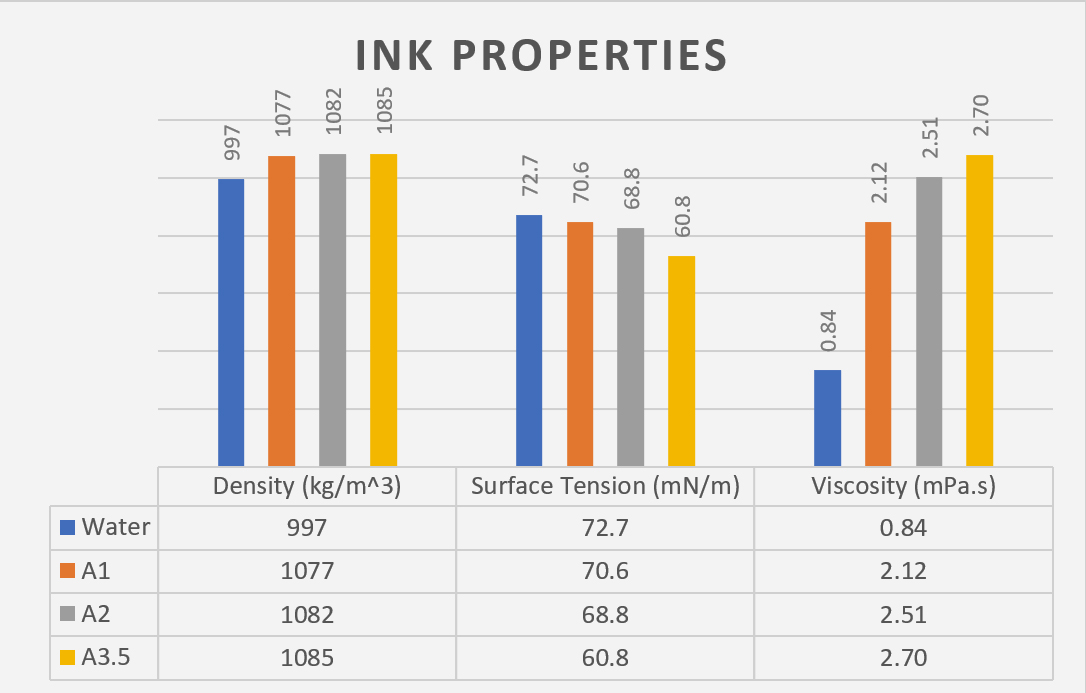
\includegraphics[width=0.8\textwidth]{grafiken/InkProps.jpg}
	\caption{Ink Properties}
	\label{fig:InkProps}
\end{figure} 

\section{Absorption Time}
The second experiment is about the absorption time of the droplets, which limits the printing time. We wanted to see whether a heat source can accelerate the absorption or not.
The Absorption times are measured at temperatures ranging from 20 to 80 deg cels.The results show that a change of 60 degrees provide a 50\% reduction in time.

\begin{figure}[h]
	\centering
	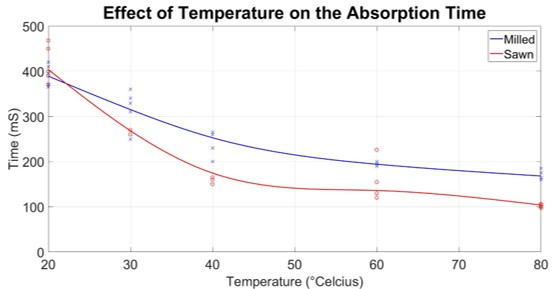
\includegraphics[width=0.8\textwidth]{grafiken/AbsorptionTime.jpg}
	\caption{Effect of heat on the absorption time}
	\label{fig:AbsorptionTime}
\end{figure} 

\section{Drop Size Selection}
The purpose of the third experiment is deciding for an adequate drop size. Depending on the drop size the drop generator is to be selected. In this figure you can see a printed zirconia specimen. Each spot on the upper half has a total ink volume of 800 nL and the ones on the bottom half 400 nL. These spots are printed using drops with volumes of 100, 50, 25 and 12.5 nL.The first image shows the spots right after printing. The second one shows the surface after furnacing.
\begin{figure}[h]
	\centering
	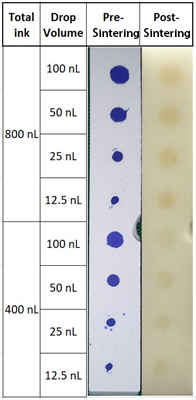
\includegraphics[width=0.4\textwidth]{grafiken/DropSize.jpg}
	\caption{Effect of the drop size on the spot area}
	\label{fig:DropSize}
\end{figure} 
A larger drop size results in shorter print duration. However they also tend to expand the spot area more compared to the smaller drops as you can see, which is bad for the resolution.The graphs show the ink intensity along the red lines and the spreading of the ink in lateral direction for each drop volume. 12.5 and 25 nL drops result in a similar spot diameter but the spots tend to get significantly larger with 50 and 100 nL Drops.
\begin{figure}[h]
	\centering
	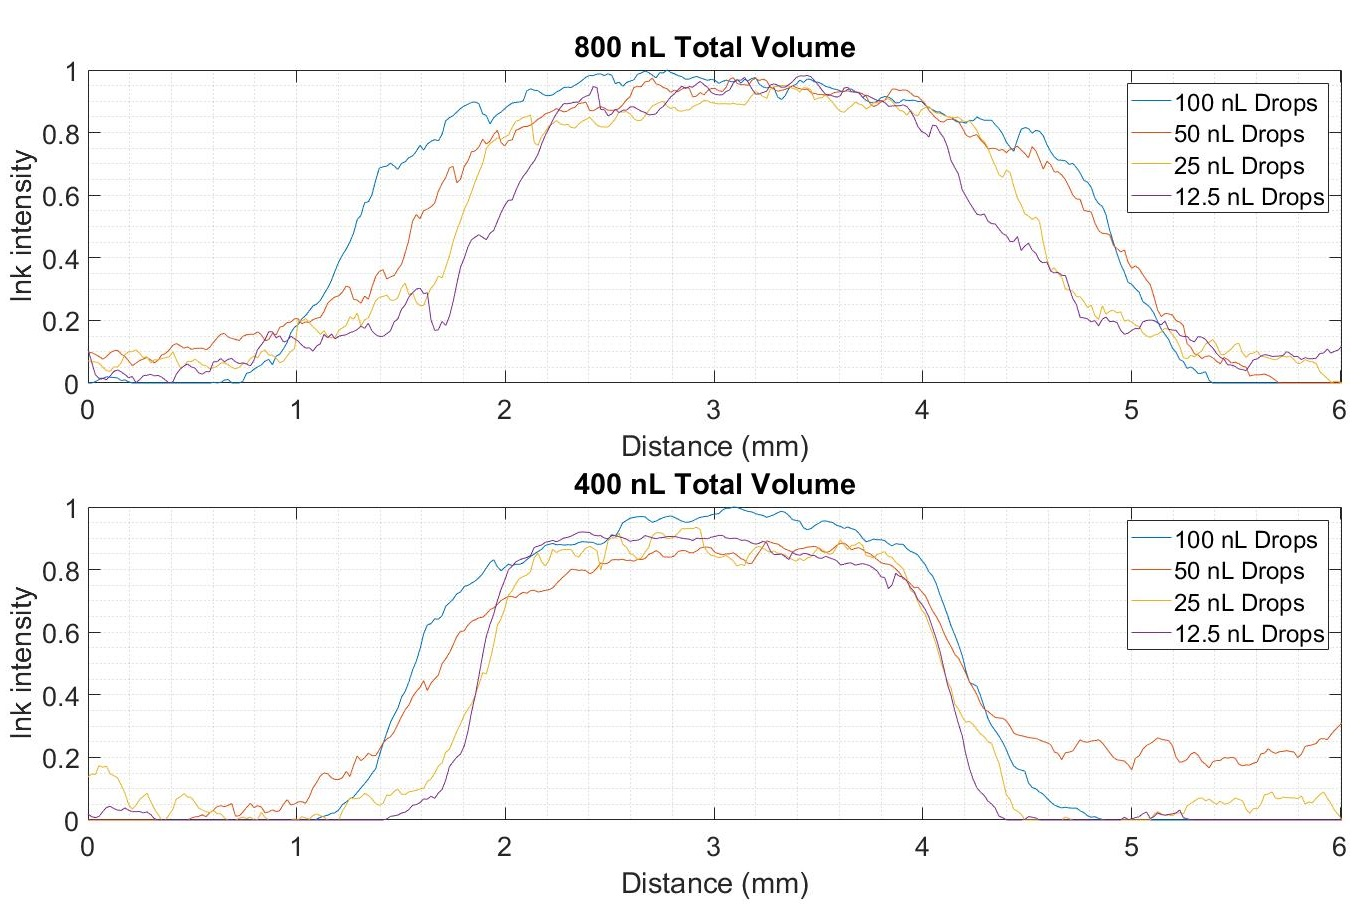
\includegraphics[width=1\textwidth]{grafiken/SpotArea.jpg}
	\caption{Comparison of the spot area results depending on the drop size}
	\label{fig:SpotArea}
\end{figure} 

\section{Point Spread Function}
The Point Spread Function and
Optical Dot Gain
Geoffrey L. Rogers
Fashion Institute of Technology, New York, NY, USA
1  Introduction
Optical dot gain, which is also known as the Yule–Nielsen effect [1–3], has a significant
effect on halftone tonality and is caused by the diffusion of photons within the paper upon
which the halftone is printed. Any physical model of halftone reflectance must take this effect
into consideration in order to accurately predict halftone color.
Because of photon diffusion within the paper, a photon may exit the paper from a point
different from that which it entered the paper. A photon may enter the paper in a region that is
void of ink and exit the paper in a region that is covered by ink so that the absorption of light
is greater than one would expect based only on dot size. There is an effective dot size that is
larger than the actual dot size \citep{rogers2015point}.




